\section{First Law of Thermodynamics}
\subsection{Specific Heat Capacity, Latent Heat}
\begin{defn}{Specific heat capacity $c$}{}
Quantity of heat required to raise the temperature of a unit mass of a substance by 1 \unit{K}.\todo{wait for lecture}
\begin{equation}
Q = mc\Delta T
\end{equation}
\end{defn}

\begin{defn}{Specific latent heat $L$}{}
\begin{equation}
Q = mL
\end{equation}
\end{defn}

\textbf{Phase change}: transition from one state of matter to another. During a phase change, latent heat is given off or absorbed, temperature of the object does not change.

\subsection{Internal Energy}
The \vocab{state} of a system is defined by its pressure $p$, volume $V$, and thermodynamic temperature $T$.\footnote{not solid, liquid or gas (there are \emph{phases}). The concept of state must be clear!}

\begin{defn}{Internal energy $U$}{}
Sum of \emph{kinetic energy} due to random motion of molecules, and \emph{potential energy} due to intermolecular forces of attraction.
\begin{equation}
U = \text{KE}_\text{random} + \text{PE}_\text{random}
\end{equation}
\end{defn}

For an ideal gas, no intermolecular attraction hence no random PE. Internal energy is only the sum of random distribution of KE of molecules.
\[ U = \text{KE}_\text{random} = N\langle\text{KE}\rangle = \frac{3}{2}Nk_BT \]
This means increase in temperature of an ideal gas indicates increase in mean random KE of molecules. This means an increase in sum of random KE, and thus increase in internal energy.

\subsection{First Law of Thermodynamics}
Work done $W$ is area under pressure-volume graph
\[ W=\int p \dd{V} \]

\begin{defn}{First Law of Thermodynamics}{}
Internal energy of a system depends only on its state. Internal energy of system is the sum of the heat supplied to system and work done on system.

\begin{equation}
\Delta U = Q_\text{to} + W_\text{on}
\end{equation}

where $\Delta U$ is the change in internal energy, $Q_\text{to}$ is heat supplied to system, $W$ is work done on the system.
\end{defn}

\subsubsection{Thermodynamic processes}
\textbf{Quasi-static process}: idealised process where the change in state is made infinitesimally slowly so that at each instant, the system can be assumed to be at a thermodynamic equilibrium with itself and with the environment.

The \textbf{state} of a system can be represented by a point on $p-V$ graph.

\textbf{Isotherm}: hyperbolic $p-V$ graph (since $pV$ is constant at constant temperature)

\begin{figure}[H]
    \centering
    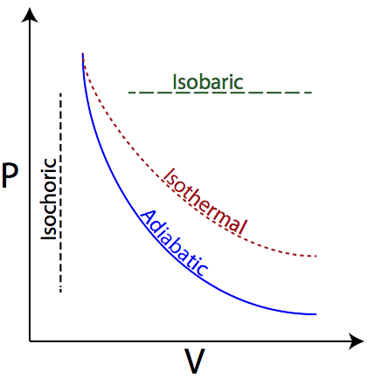
\includegraphics[width=0.5\textwidth]{images/thermodynamic_processes.png}
\end{figure}

\begin{itemize}
\item \vocab{Isothermal} expansion/contraction: \textbf{constant temperature}

Change in state occurs along an isotherm. Constant temperature implies constant mean random KE and hence constant total random KE of molecules. For an ideal gas, it means constant internal energy.

Both $p$ and $V$ change, but $pV$ is constant.

$\Delta U=0$

\item \vocab{Isobaric} expansion/contraction: \textbf{constant pressure}

Constant pressure means system's environment is not changing e.g. system experiences atmospheric pressure.

Final state is on a different isotherm, meaning temperature changes. Volume of changes.

Work done by system $=-W=p\Delta V$

\item \vocab{Isochoric} heating/cooling: \textbf{constant volume}

Constant volume means system is confined in a rigid container, implying zero work done by and on the system. 

Final state is on a different isotherm, meaning the temperature changes. Pressure also changes.

$W=0$

\item \vocab{Adiabatic} expansion/contraction: \textbf{no heat exchange between system and environment}

During adiabatic expansion, system does work by pushing back its environment. Since no heat is supplied to system for it to do the work, it uses its thermal energy, thus temperature decreases.

Final state is at lower isotherm than initial state. Pressure also decreases.

Paths for adiabatic changes are steeper than isotherms.

$Q=0$
\end{itemize}

Temperature change - $\Delta U$ change

Volume change - $W$ done


\textbf{Cyclic process}: system starts and ends with same state, no change in internal energy

% https://superphysics.sg/wp-content/uploads/2019/09/H2-Chapter-11-Thermal-Physics-Summary.pdf
\pagebreak